\lab{GeoPandas}{GeoPandas}
\labdependencies{Pandas1,Pandas2}

\objective{GeoPandas is a package designed to organize and manipulate geographic data. It combines the data manipulation tools of pandas with the geometric capabilities of the Shapely package. In this lab, we explore the basic data structures of GeoSeries and GeoDataFrames and their functionalities.}


\section*{Installation} %============================
GeoPandas is a new package designed to combine the functionality of pandas with Shapely, a package used for geometric manipulation.
Using GeoPandas with geographic data is very useful as it allows the user to not only compare numerical data, but also geometric attributes.
GeoPandas can be installed via \li{pip}:
\begin{lstlisting}
>>> pip install geopandas
\end{lstlisting}

\section*{GeoSeries} %============================

A GeoSeries is a pandas Series where each entry is a set of geometric objects.
There are three classes of geometric objects inherited from the Shapely package:
\begin{enumerate}
\item Points / Multi-Points
\item Lines / Multi-Lines
\item Polygons / Multi-Polygons
\end{enumerate}
A point is used to identify objects like coordinates, where there is one small instance of the object.
A line could be used to describe objects such as roads.
A polygon could be used to identify regions, such as a country.
Multipoints, multilines, and multipolygons contain lists of points, lines, and polygons, respectively.

Since each object in the GeoSeries is also a Shapely object, the GeoSeries inherits many methods and attributes of Shapely objects.
Some of the key attributes and methods are listed in Table \ref{shapely-methods}.
These attributes and methods can be used to calculate distances, find the sizes of countries, and determine whether coordinates are within country's boundaries.
The example below uses the attribute \li{bounds} to find the maximum and minimum coordinates of Egypt in the GeoDataFrame \li{worldmap.gpkg}.

\begin{table}[ht]
\begin{center}
\begin{tabular}{c|c}
Method/Attribute & Description\\
\hline
\li{distance(other)}&returns minimum distance from GeoSeries to \li{other}\\
\li{contains(other)}&returns \li{True} if shape contains \li{other}\\
\li{intersects(other)}&returns \li{True} if shape intersects \li{other}\\
\li{area}&returns shape area\\
\li{convex_hull}&returns convex shape around all points in the object\\
\li{bounds} &  returns the bounding x- and y-coordinates of the object
\end{tabular}
\end{center}
\caption{Attributes and Methods for GeoSeries}
\label{shapely-methods}
\end{table}

\begin{lstlisting}
>>> import geopandas as gpd
>>> world = gpd.read_file(worldmap.gpkg)
# Get GeoSeries for Egypt
>>> egypt = world[world["SOVEREIGNT"]=="Egypt"]

# Find bounds of Egypt
>>> egypt.bounds
         minx    miny         maxx      maxy
163   24.70007    22.0     36.86623  31.58568
\end{lstlisting}

\section*{Creating GeoDataFrames} %============================

The main structure used in GeoPandas is a GeoDataFrame, which is similar to a pandas DataFrame.
A GeoDataFrame has one special column called \li{geometry}, which must be a GeoSeries.
This GeoSeries column is used when a spatial method, like \li{distance()}, is used on the GeoDataFrame.
Therefore all attributes and methods used for GeoSeries can also be used on GeoDataFrame objects.

A GeoDataFrame can be made from a pandas DataFrame.
One of the columns in the DataFrame should contain geometric information.
That column can be converted to a GeoSeries using the \li{apply()} method.
At this point, the Pandas DataFrame can be cast as a GeoDataFrame.
Assign which column will be the \li{geometry} using either the \li{geometry} keyword in the constructor or the \li{set_geometry()} method afterwards.

\begin{lstlisting}
>>> import pandas as pd
>>> import geopandas as gpd
>>> from shapely.geometry import Point, Polygon

# Create a Pandas DataFrame
>>> df = pd.DataFrame({"City": ["Seoul", "Lima", "Johannesburg"],
...                   "Country": ["South Korea", "Peru", "South Africa"],
...                   "Latitude": [37.57, -12.05, -26.20],
...                   "Longitude": [126.98, -77.04, 28.04]})

# Create geometry column
>>> df["Coordinates"] = list(zip(df.Longitude, df.Latitude))

# Make geometry column Shapely objects
>>> df["Coordinates"] = df["Coordinates"].apply(Point)

# Cast as GeoDataFrame
>>> gdf = gpd.GeoDataFrame(df, geometry="Coordinates")

# Equivalently, specify the geometry after construction
# Note that set_geometry() returns a new GeoDataFrame
>>> gdf = gpd.GeoDataFrame(df)
>>> gdf = gdf.set_geometry("Coordinates")

# Display the GeoDataFrame
>>> gdf
           City       Country  Latitude  Longitude                  Coordinates
0         Seoul   South Korea     37.57     126.98   POINT (126.98000 37.57000)
1          Lima          Peru    -12.05     -77.04  POINT (-77.04000 -12.05000)
2  Johannesburg  South Africa    -26.20      28.04   POINT (28.04000 -26.20000)

# Create a polygon with all three cities as points
>>> city_polygon = Polygon(list(zip(df.Longitude, df.Latitude)))
\end{lstlisting}

A \li{GeoDataFrame} can also be made directly from a dictionary.
If the dictionary already contains geometric objects, the corresponding column can be directly set as the \li{geometry} in the constructor.
Otherwise, a column containing geometry data can be created as in the above example and then set as the \li{geometry} with the \li{set_geometry()} method.

\begin{lstlisting}
# Both of these methods create the same GeoDataFrame as above
# Directly create the GeoDataFrame from the dictionary
>>> gdf = gpd.GeoDataFrame({"City": ["Seoul", "Lima", "Johannesburg"],
...                   "Country": ["South Korea", "Peru", "South Africa"],
...                   "Latitude": [37.57, -12.05, -26.20],
...                   "Longitude": [126.98, -77.04, 28.04]})
# Create geometry column and set as the geometry
>>> gdf["Coordinates"] = list(zip(gdf.Longitude, gdf.Latitude))
>>> gdf["Coordinates"] = gdf["Coordinates"].apply(Point)
# inplace=True modifies gdf itself rather than returning a copy
>>> gdf.set_geometry("Coordinates", inplace=True)

# Equivalently, using a dictionary that already contains geometry objects
>>> gdf = gpd.GeoDataFrame({"City": ["Seoul", "Lima", "Johannesburg"],
...                   "Country": ["South Korea", "Peru", "South Africa"],
...                   "Coordinates": [Point(126.98, 37.57),
...                       Point(-77.04, -12.05), Point(28.04, -12.05)]},
...                   geometry="Coordinates")
\end{lstlisting}

\begin{table}[ht]
\begin{center}
\begin{tabular}{c|c}
Method/Attribute & Description\\
\hline
\li{abs()}&returns series/dataframe with absolute numeric value of each element\\
\li{add(other)}&returns addition of dataframe and \li{other} element-wise\\
\li{affine_transform(matrix)}&returns \li{GeoSeries} with translated geometries\\
\li{append(other)}&returns new object with appended rows of \li{other} to the end of caller\\
\li{dot(other)}&returns dataframe of matrix multiplication with \li{other}\\
\li{equals(other)} &tests if the two objects contain the same elements
\end{tabular}
\end{center}
\caption{Attributes and Methods for GeoDataFrame}
\label{shapely-methods2}
\end{table}

\begin{info}
Longitude is the angular measurement starting at the Prime Meridian, $0\degree$, and going to $180\degree$ to the east and $-180\degree$ to the west.
Latitude is the angle between the equatorial plane and the normal line at a given point; a point along the Equator has latitude $0$, the North Pole has latitude $+90\degree$ or $90\degree N$, and the South Pole has latitude $-90\degree$ or $90\degree S$.
\end{info}

\section*{Plotting GeoDataFrames} %============================

Information from a GeoDataFrame is plotted based on the geometry column.
Data points are displayed as geometry objects.
The following example plots the shapes in the \li{world} GeoDataFrame.

\begin{lstlisting}
# Plot world GeoDataFrame
>>> world.plot()
\end{lstlisting}

\begin{figure}[H]
\begin{center}
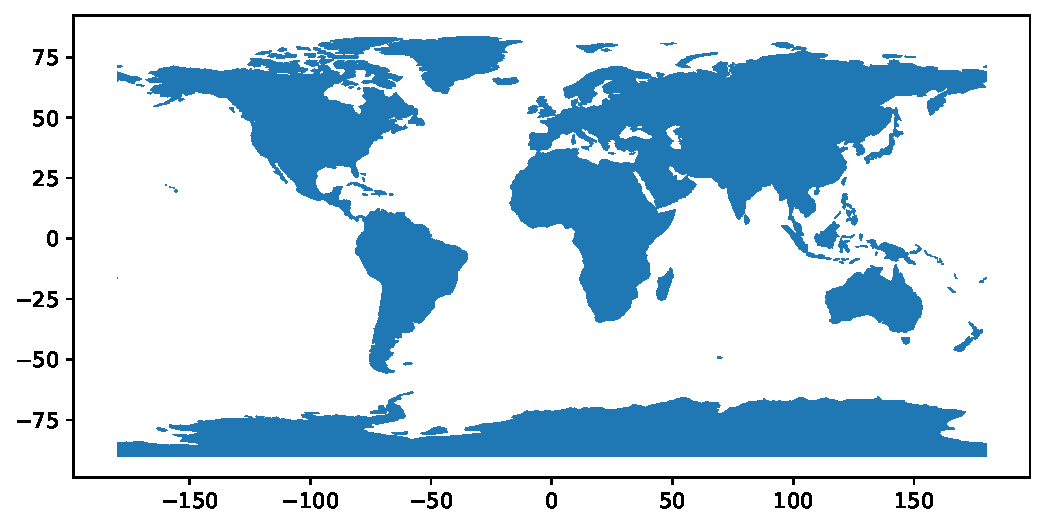
\includegraphics[scale=.7]{figures/worldmap.pdf}
\end{center}
\label{world-map}
\caption{World map}
\end{figure}

Multiple GeoDataFrames can be plotted at once.
This can be done by by setting one GeoDataFrame as the base of the plot and ensuring that each layer uses the same axes.
In the following example, the file \li{airports.csv}, containing the coordinates of world airports, is loaded into a GeoDataFrame and plotted on top of the boundary of the \li{world} GeoDataFrame.

\begin{lstlisting}
# Set outline of world countries as base
>>> fig, ax = plt.subplots(1, figsize=(10, 4))
>>> base = world.boundary.plot(edgecolor="black", ax=ax, linewidth=1)

# Load airport data and convert to a GeoDataFrame
>>> airports = pd.read_csv("airports.csv")
>>> airports["Coordinates"] = list(zip(airports.Longitude, airports.Latitude))
>>> airports["Coordinates"] = airports.Coordinates.apply(Point)
>>> airports = gpd.GeoDataFrame(airports, geometry="Coordinates")

# Plot airports on top of world map
>>> airports.plot(ax=base, marker='o', color="green", markersize=1)
>>> ax.set_xlabel("Longitude")
>>> ax.set_ylabel("Latitude")
>>> ax.set_title("World Airports")
\end{lstlisting}

\begin{figure}[H]
\begin{center}
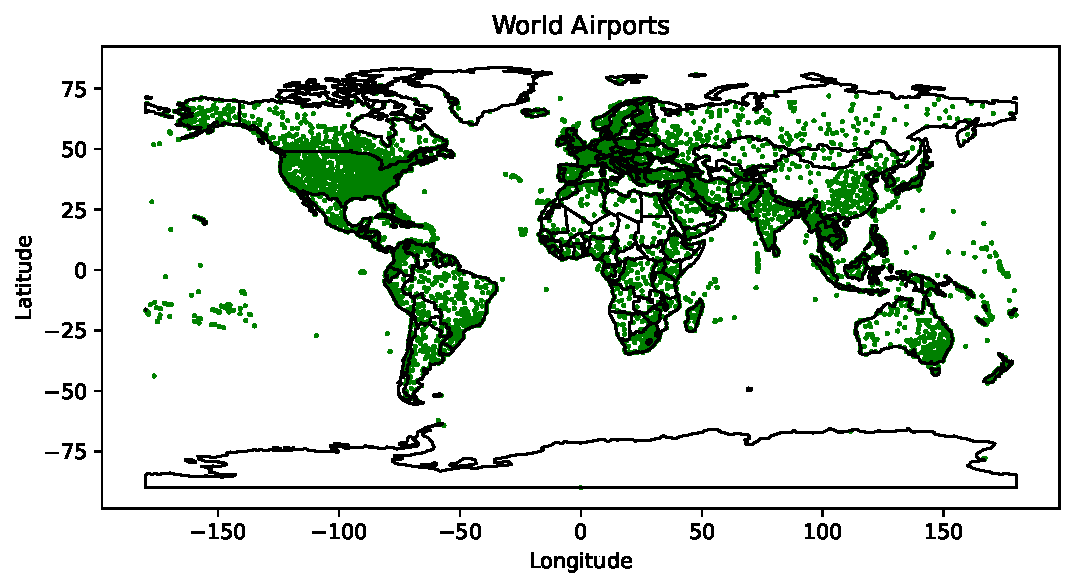
\includegraphics[scale=.7]{figures/airports.pdf}
\end{center}
\label{airport-map}
\caption{Airport map}
\end{figure}

\begin{problem}
The file \li{worldmap.gpkg.zip} contains data of the worldmap used in above examples.\footnote{Source: \url{https://www.naturalearthdata.com/downloads/110m-cultural-vectors/}}
After unzipping, use the command \li{geopandas.read_file("worldmap.gpkg")} to create a GeoDataFrame of this information.

Then, read in the file \li{airports.csv} as a pandas DataFrame.
Create three convex hulls around the three sets of airports listed below.
This can be done by passing in lists of the airports' coordinates (Longitude and Latitude zipped together) to a \li{shapely.geometry.Polygon} object.

Finally, create a new GeoDataFrame using a dictionary with key \li{"geometry"} and with a list of these three Polygons as the value.
Plot this GeoDataFrame, and then plot the outlined world map on top of it.

\begin{itemize} %These could also be listed by 4-character ICAO codes, but listing the names makes the problem more exciting/realistic. Probably.
	\item Maio Airport, Scatsta Airport, Stokmarknes Skagen Airport, Bekily Airport, K. D. Matanzima Airport, RAF Ascension Island
	\item Oiapoque Airport, Maio Airport, Zhezkazgan Airport, Walton Airport, RAF Ascension Island, Usiminas Airport, Piloto Osvaldo Marques Dias Airport
	\item Zhezkazgan Airport, Khanty Mansiysk Airport, Novy Urengoy Airport, Kalay Airport, Biju Patnaik Airport, Walton Airport
\end{itemize}
\end{problem}

\begin{info}
\li{.gpkg} files are actually structured as a directory that contains several files that each contain parts of the data.
For instance, \li{worldmap.gpkg} consists of the files \li{worldmap.cpg}, \li{worldmap.dbf}, \li{worldmap.prj}, \li{worldmap.shp}, and \li{worldmap.shx}.
Be sure that these files are placed directly in the first level of \li{worldmap.gpkg}, and not in further subdirectories.\\
\end{info}

\section*{Working with GeoDataFrames} %============================

As previously mentioned, GeoDataFrames contain many of the functionalities of pandas DataFrames.
For example, to create a new column, define a new column name in the GeoDataFrame with the needed information for each GeoSeries.

\begin{lstlisting}
# Create column in the world GeoDataFrame for GDP_PER_CAPITA
>>> world["GDP_PER_CAP"] = world.GDP_MD / world.POP_EST
\end{lstlisting}

GeoDataFrames can utilize many pandas functionalities, and they can also be parsed by geometric manipulations.
For example, a useful way to index GeoDataFrames is with the \li{cx} indexer.
This splits the GeoDataFrame by the coordinates of each geometric object.
It is used by calling the method \li{cx} on a GeoDataFrame, followed by a slicing argument, where the first element refers to the longitude and the second refers to latitude.

\begin{lstlisting}
# Create a GeoDataFrame containing the northern hemisphere
>>> north = world.cx[:, 0:]

# Create a GeoDataFrame containing the southeastern hemisphere
>>> south_east = world.cx[0:, :0]
\end{lstlisting}

GeoSeries objects in a GeoDataFrame can also be dissolved, or merged, together into one GeoSeries based on their geometry data.
For example, all countries on one continent could be merged to create a GeoSeries containing the information of that continent.
The method designed for this is called \li{dissolve}.
It receives two parameters, \li{by} and \li{aggfunc}.
\li{by} indicates which column to dissolve along, and \li{aggfunc} tells how to combine the information in all other columns.
The default \li{aggfunc} is \li{first}, which returns the first application entry.
In the following example, we use \li{sum} as the \li{aggfunc} so that each continent is the combination of its countries.

\begin{lstlisting}
>>> world = world[["CONTINENT", "geometry", "GDP_PER_CAP"]]

# Dissolve world GeoDataFrame by continent
>>> continent = world.dissolve(by="CONTINENT", aggfunc="sum")
\end{lstlisting}


\section*{Projections and Coloring} %============================

When plotting, GeoPandas uses the CRS (coordinate reference system) of a GeoDataFrame.
This reference system indicates how coordinates should be spaced on a plot.
Two of the most commonly used CRSs are EPSG:4326 and EPSG:3395.
EPSG:4326 is the standard latitude-longitude projection used by GPS.
EPSG:3395, also known as the Mercator projection, is the standard navigational projection.

When creating a new GeoDataFrame, it is important to set the \li{crs} attribute of the GeoDataFrame.
This allows any plots to be shown correctly.
Furthermore, GeoDataFrames being layered need to have the same CRS.
To change the CRS, use the method \li{to_crs()}.

\begin{lstlisting}
# Check CRS of world GeoDataFrame
>>> print(world.crs)
EPSG:4326

# Change CRS of world to Mercator
# inplace=True ensures that we modify world instead of returning a copy
>>> world.to_crs(3395, inplace=True)
>>> print(world.crs)
EPSG:3395
\end{lstlisting}

GeoPandas accepts many different CRSs; a reference can be found at \url{www.spatialreference.org}.
% I think this is helpful information, but I'm not sure
Additionally, inspecting a given CRS object in the terminal without using \li{print()} or \li{str()} can be used to get additional information about a specific CRS:\footnote{This can also be accomplished using \li{print(repr(crs))}.}
\begin{lstlisting}[mathescape]
>>> world.crs
<Projected CRS: EPSG:3395>
Name: WGS 84 / World Mercator
Axis Info [cartesian]:
- E[east]: Easting (metre)
- N[north]: Northing (metre)
Area of Use:
- name: World between 80$^\circ$S and 84$^\circ$N.
- bounds: (-180.0, -80.0, 180.0, 84.0)
Coordinate Operation:
- name: World Mercator
- method: Mercator (variant A)
Datum: World Geodetic System 1984
- Ellipsoid: WGS 84
- Prime Meridian: Greenwich
\end{lstlisting}

GeoDataFrames can also be plotted using the values in the other attributes of the GeoSeries.
The map plots the color of each geometry object according to the value of the column selected.
This is done by passing in the parameter \li{column} into the \li{plot()} method.

\begin{lstlisting}
>>> fig, ax = plt.subplots(1, figsize=(10, 4))
# Plot world based on gdp
>>> world.plot(column="GDP_MD", cmap="OrRd", legend=True,  ax=ax)
>>> ax.set_title("World Map based on GDP")
>>> ax.set_xlabel("Longitude")
>>> ax.set_ylabel("Latitude")
>>> plt.show()
\end{lstlisting}

\begin{figure}[H]
\begin{center}
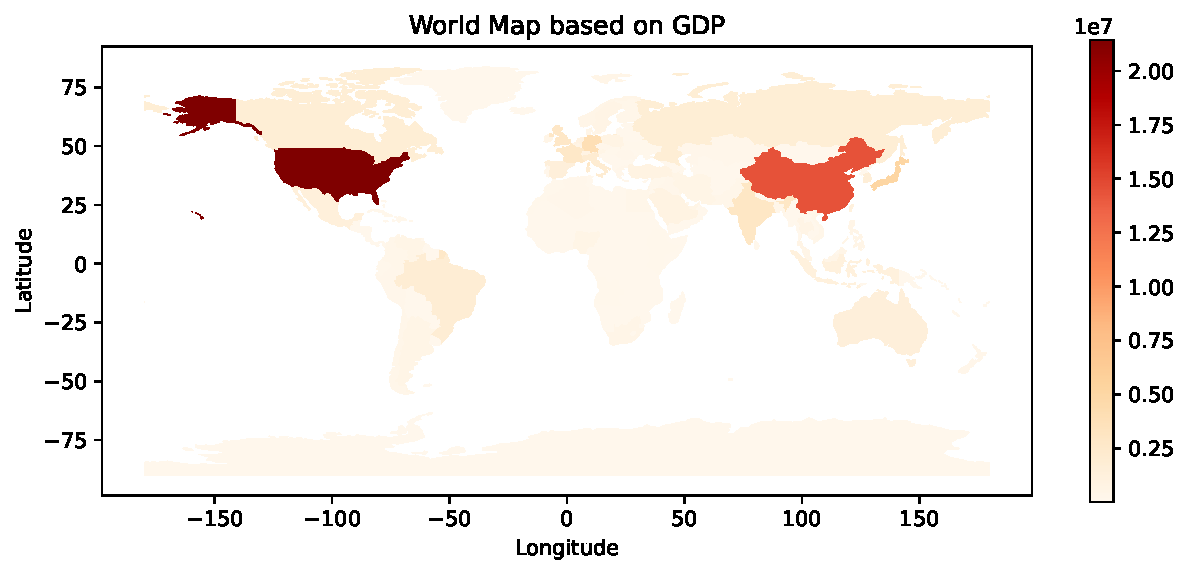
\includegraphics[scale=.7]{figures/gdp.pdf}
\end{center}
\caption{World Map Based on GDP}
\label{figure:gdp_map}
\end{figure}


\begin{problem}
The file \li{county_data.gpkg.zip} contains information about US counties.\footnote{Source: \url{http://www2.census.gov/geo/tiger/GENZ2016/shp/cb_2016_us_county_5m.zip}}
After unzipping, use the command \li{geopandas.read_file("county_data.gpkg")} to create a GeoDataFrame of this information.
Each county's shape is stored in the \li{geometry} column.
Use this to plot the boundaries of all US counties two times, first using the default CRS and then using EPSG:5071.

Next, create a new GeoDataFrame that combines (\li{dissolve}) all counties within each state (\li{by="STATEFP"}).
Drop regions with the following STATEFP codes: 02, 15, 60, 66, 69, 72, 78.
Plot the boundary of this GeoDataFrame to see an outline of all 48 contiguous states.
Ensure a CRS of EPSG:5071.
\label{problem:us_counties}
\end{problem}


\section*{Merging GeoDataFrames} %============================

Just as multiple pandas DataFrames can be merged, multiple GeoDataFrames can be merged with attribute joins or spatial joins.
An attribute join is similar to a merge in pandas.
It combines two GeoDataFrames on a column (not the geometry column) and then combines the rest of the data into one GeoDataFrame.

\begin{lstlisting}
>>> world = gpd.read_file(worldmap.gpkg)
>>> cities = gpd.read_file(cities.gpkg)

# Create subsets of the world and cities GeoDataFrames
>>> world = world[["CONTINENT", "SOVEREIGNT", "SOV_A3"]]
>>> cities = cities[["NAME", "SOV_A3"]]

# Merge the GeoDataFrames on their SOV_A3 code
>>> countries = world.merge(cities, on="SOV_A3")
\end{lstlisting}

A spatial join merges two GeoDataFrames based on their geometry data.
The function used for this is \li{sjoin}.
\li{sjoin} accepts two GeoDataFrames and then direction on how to merge.
It is imperative that two GeoDataFrames have the same CRS.
In the example below, we merge using an \li{inner} join with the option \li{intersects}.
The \li{inner} join means that we will only use keys in the intersection of both geometry columns, and we will retain only the left geometry column.
\li{intersects} tells the GeoDataFrames to merge on GeoSeries that intersect each other.
Other options include \li{contains} and \li{within}.

\begin{lstlisting}
# Combine countries and cities on their geographic location
>>> countries = gpd.sjoin(world, cities, how="inner", predicate="intersects")
\end{lstlisting}

\begin{problem}
Load in the file \li{nytimes.csv}\footnote{Source: \url{https://raw.githubusercontent.com/nytimes/covid-19-data/master/us-counties.csv}} as a Pandas DataFrame.
This file includes county-level data for the cumulative cases and deaths of Covid-19 in the US, starting with the first case in Snohomish County, Washington, on January 21, 2020.

Merge the county GeoDataFrame from \li{county_data.gpkg} with the \li{nytimes} DataFrame on the county \li{fips} codes (a FIPS code is a 5-digit unique identifier for geographic locations).
Note that the \li{fips} column of the \li{nytimes} DataFrame stores entries as floats, but the county GeoDataFrame stores FIPS codes as strings, with the first two digits in the \li{STATEFP} column and the last three digits in the \li{COUNTYFP} column.
Thus, you will need to add these two columns together and then convert them into floats so they can be merged with the \li{fips} column in the \li{nytimes} DataFrame.

Drop the regions from the county GeoDataFrame with the same \li{STATEFP} codes as in Problem \ref{problem:us_counties}.
Also, make sure to change the CRS of the county GeoDataFrame to EPSG:5071 \emph{before} you merge the two DataFrames (this will make the code run much faster).

Plot the cases from March 21, 2020, and then plot your state outline map from Problem \ref{problem:us_counties} on top of that (with a CRS of EPSG:5071).
Include a colorbar using the arguments \li{legend=True} and \li{cmap="plasma_r"} in the \li{plot} function.
Finally, print out the name of the county with the most cases on March 21, 2020, along with its case count.

\noindent Hint: every state should have multiple covid cases.
\label{problem:merge_covid}
\end{problem}

\section*{Logarithmic Plotting Techniques} %============================

The color scheme of a graph can also help to communicate information clearly.
A good list of available colormaps can be found at \url{https://matplotlib.org/3.2.1/gallery/color/colormap_reference.html}.
Note also that you can reverse any colormap by adding \li{_r} to the end.
The following example demonstrates some plotting features, using country GDP as in Figure \ref{figure:gdp_map}.

\begin{lstlisting}
>>> fig, ax = plt.subplots(1, figsize=(10, 4))
>>> world.plot(column="GDP_MD", cmap="plasma_r",
...			ax=ax, legend=True, edgecolor="gray")

# Add title and remove axis tick marks
>>> ax.set_title("GDP on Linear Scale")
>>> ax.set_yticks([])
>>> ax.set_xticks([])
>>> plt.show()
\end{lstlisting}

\begin{figure}[H]
\begin{center}
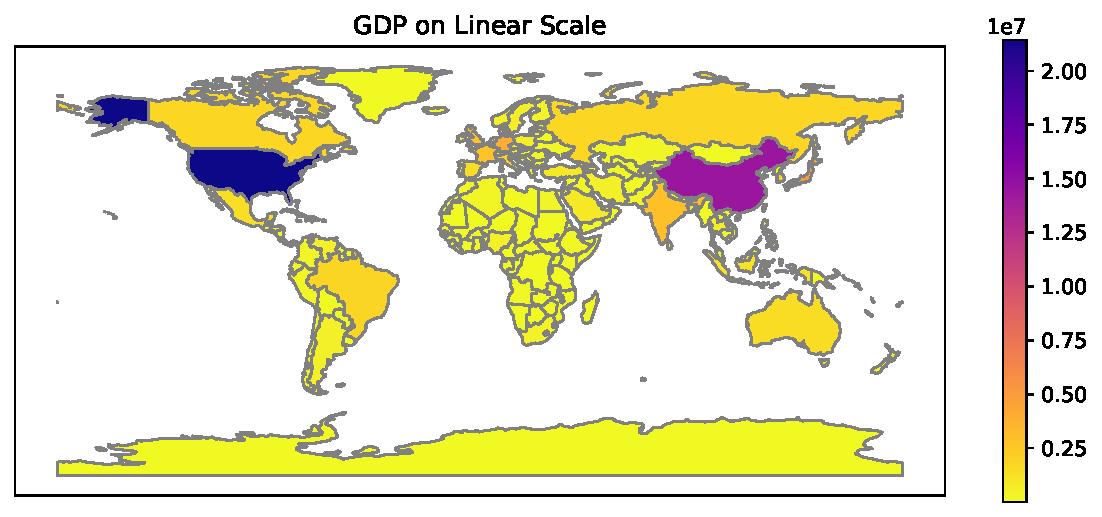
\includegraphics[scale=.7]{figures/world_linear.pdf}
\end{center}
\caption{World map showing country GDP}
\label{figure:linear_world}
\end{figure}

Sometimes data can be much more informative when plotted on a logarithmic scale.
See how the world map changes when we add a \li{norm} argument in the code below.
Depending on the purpose of the graph, Figure \ref{figure:log_world} may be more informative than Figure \ref{figure:linear_world}.

\begin{lstlisting}
>>> from matplotlib.colors import LogNorm
>>> from matplotlib.cm import ScalarMappable
>>> fig, ax = plt.subplots(1, figsize=(10, 7))

# Set the norm using data bounds
>>> data = world.GDP_MD
>>> norm = LogNorm(vmin=min(data), vmax=max(data))

# Plot the graph using the norm
>>> world.plot(column="GDP_MD", cmap="plasma_r", ax=ax,
...			edgecolor="gray", norm=norm)

# Create a custom colorbar
>>> cbar = fig.colorbar(ScalarMappable(norm=norm, cmap="plasma_r"),
...			ax=ax, orientation="horizontal", pad=0, label="GDP")

>>> ax.set_title("GDP on a Log Scale")
>>> ax.set_yticks([])
>>> ax.set_xticks([])
>>> plt.show()
\end{lstlisting}

\begin{figure}[H]
\begin{center}
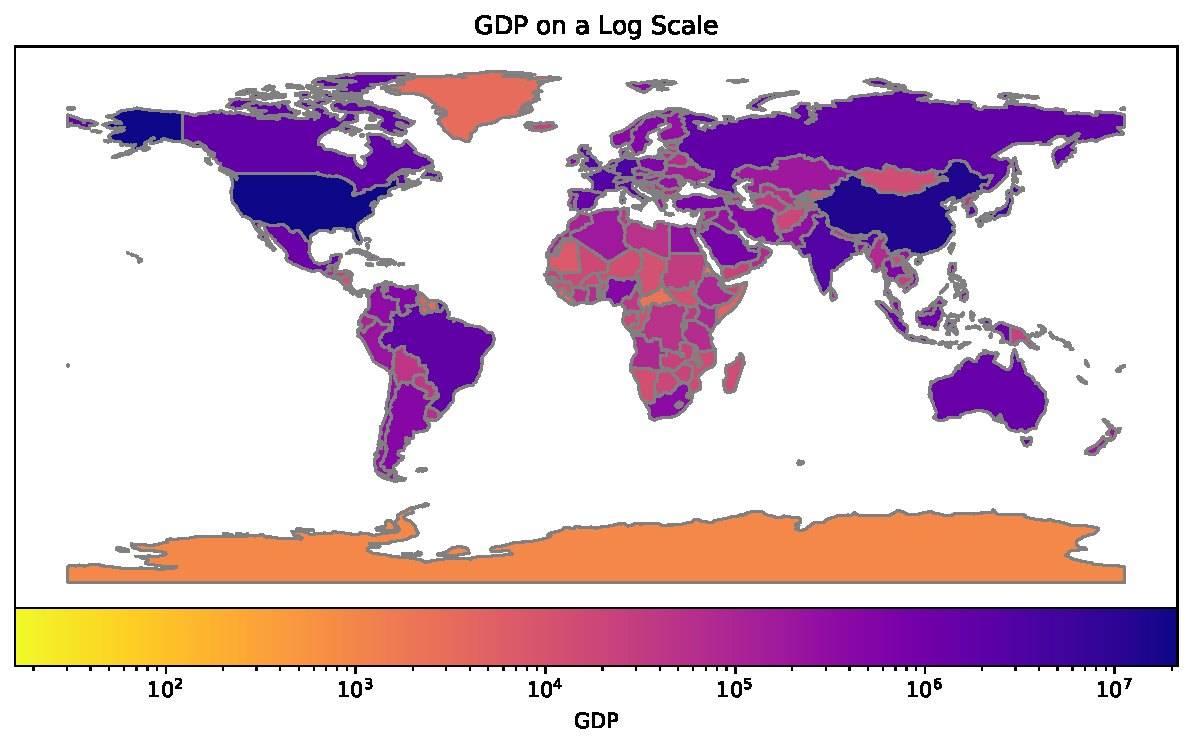
\includegraphics[scale=.7]{figures/world_log.pdf}
\end{center}
\caption{World map showing country GDP using a log scale}
\label{figure:log_world}
\end{figure}

\begin{problem}
As in Problem \ref{problem:merge_covid}, plot your state outline map from Problem \ref{problem:us_counties} on top of a map of Covid-19 cases from March 21, 2020 (each with a CRS of EPSG:5071).
This time, however, use a log scale.
Pick a good colormap (the counties with the most cases should generally be darkest) and be sure to display a colorbar.
\label{problem:log_plot}
\end{problem}

\begin{problem}
In this problem, you will create an animation of the spread of Covid-19 through US counties from January 21, 2020, through June 21, 2020.
You will use the same GeoDataFrame you used in Problems \ref{problem:merge_covid} and \ref{problem:log_plot} (with a CRS of EPSG:5071).
Use a log scale and a good colormap, and be sure that you're using the same norm and colorbar for the whole animation.

As a reminder, below is a summary of what you will need in order to animate this map.
You may also find it helpful to refer to the animation section included with the Volume 4 lab manual.

\begin{enumerate}
	\item Set up your figure and norm. Be sure to use the highest case count for your \li{vmax} so that the scale remains uniform.
	\item Write your \li{update} function. This should plot the cases from a given day as well as the state boundaries.
	\item Set up your colorbar. Do this outside the \li{update} function to avoid adding a new colorbar each day.
	\item Create a \li{FuncAnimation} object. Check to make sure everything displays properly before you save it.
	\item Save the animation to a file, and embed it into the notebook.
\end{enumerate}
\end{problem}
